\documentclass[12pt,a4paper]{article}
\usepackage[english, science, large]{../template/ku-frontpage}
\usepackage{tabularx}
\usepackage{ltablex}
\usepackage{minted}
\setminted[text]{
frame=lines,
framesep=2mm,
baselinestretch=1.1,
fontsize=\footnotesize,
linenos,
breaklines}
\hypersetup{
    colorlinks=false,
    pdfborder={0 0 0},
}
\begin{document}
\title{ACS Programming Assignment 2}
\subtitle{}

\author{Kai Arne S. Myklebust, Silvan Adrian}
\date{Handed in: \today}
	
\maketitle
\tableofcontents

\section{Setup}
For data generation we used as much as randomization as possible, we even used a data faker (\texttt{java-faker}) for test data which makes more sense and not just some random strings for author and title (no specific length).
The other attributes we filled by the \texttt{Radnom} class which allowed us to generate some useful test data for floats, doubles etc.
Overall we generate 1000 books for the database which have ISBNs from 1 to 1000, while for the interactions we used random ISBNs from (1 to 2000) so that there will be sometimes overlapping books (already existing in the database) and otherwise still have to be added to the database.
To be able to distinguish between random and not random ISBNs we had to add a parameter to \texttt{BookSetGenerator} which allows us to configure it as wanted.

We ran the experiments on a single machine with Mac OSX, 16 GB of RAM and an Intel Core i7 with 4 Cores (8 threads).

For measurements we changed the amount of concurrent clients to be able to plot some sort of statistics which wouldn't be possible with single client runs.

\section{Throughput and Latency plots}

Well first of all we see that the latency for RPC calls is higher then the one for local ones, which is understandable since the calls have to be done via HTTP which matches with our expectation.
\begin{figure}[htb!]
	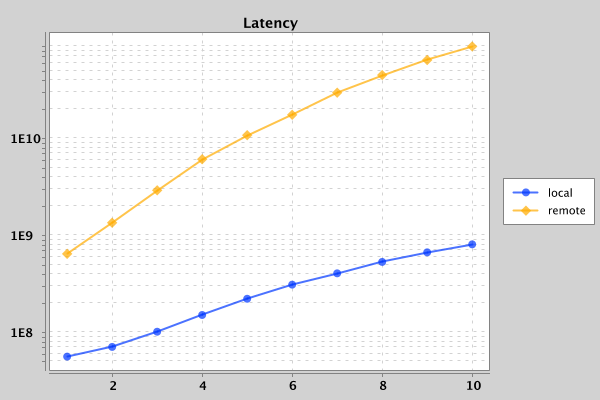
\includegraphics[width=\textwidth]{latency_chart}
	\caption{Latency Chart}
\end{figure}


For throughput on the other hand the RPC calls gare better then the local ones, even with a higher amount of clients the throughput only increases slowly for RPC calls.
So we suspect by using the serialization via the bookProxy or storeProxy and the parallelization of sending data, we get better metric for RPC calls.
With that knowledge then the plot pretty much also fits our expectations.

\begin{figure}[htb!]
	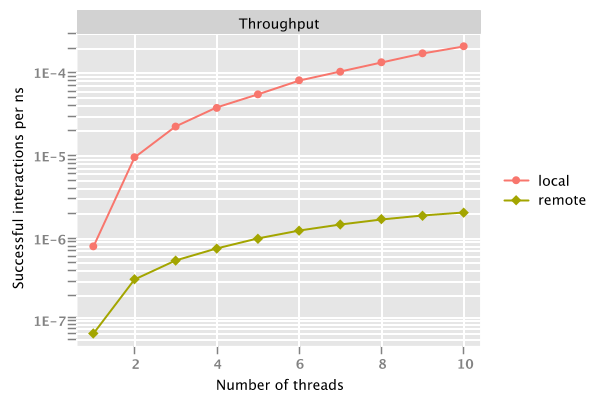
\includegraphics[width=\textwidth]{throughput_chart}
	\caption{Throughput chart}
\end{figure}
\newpage
\section{Reliability}
Since we don't have any knowledge of what would be a possible workload on the book store and our interactions more or less just try to imitate possible workloads they won't be very helpful for real world workloads.
but with the metrics we at least have a possible starting point to go on.

What would be nice to see the more interactions and clients there are how many interactions are not successful anymore, especially if it would get worse the more clients get added which would be nice to know.
\end{document}